\section{Design}
\label{sec:design}


Current workflow used by developers to run DL jobs is as shown in Figure 1.
However when multiple users try to access the cluster, we need a scheduler to
manage the job queue. A naive approach, treating GPUs in integer granularity,
would simply keep a count of free GPUs (a Resource Manager), and allot as many
GPUs as the incoming job requires. The number is updated every time a job enters
of leaves the cluster. 

However, to make fine grained use of the GPUs, we must have the ability to split
an incoming job among the residual resources left in the cluster. Accordingly,
the model splitting routine sits between the job queue and the cluster
controller. Figure 3 shows the high level design of the system.

\subsection{Big Brain Job Operator}

The interface for our system is managed almost entirely through Kubernetes and
other popular, well-established cluster management systems. Specifically, we use
the Kubernetes Operators pattern to implement our job management pipeline. This
architecure is illustrated in \ref{fig:architecure}.


We define \texttt{BBJob} as a Kubernetes Custom Resource Definition (CRD) that represents a
Big Brain job. The \texttt{BBJob} specification contains the bare minimum
required to build a container that can launch a training loop for a machine
learning model.

Once the operator receives a \texttt{BBJob}, it performs a quick profiling and
placement step to determine the best node and GPUs to run the job on. The
operator then generates a pod and pushes a new conatiner to the cluster registry
for future reference. While we do not perform any intellgent caching of models,
datasets, etc. yet, this is a future enhancement.

Once the pod is running, the operator will monitor it and update the state of
the corersponding \texttt{BBJob}. When the job is run to complete or is killed
due to an error, the operator will invoke a \texttt{BBJob} delete callback that
can be handled by the developer or client library. 

\label{fig:architecure}
\begin{figure}[htbp]
\centerline{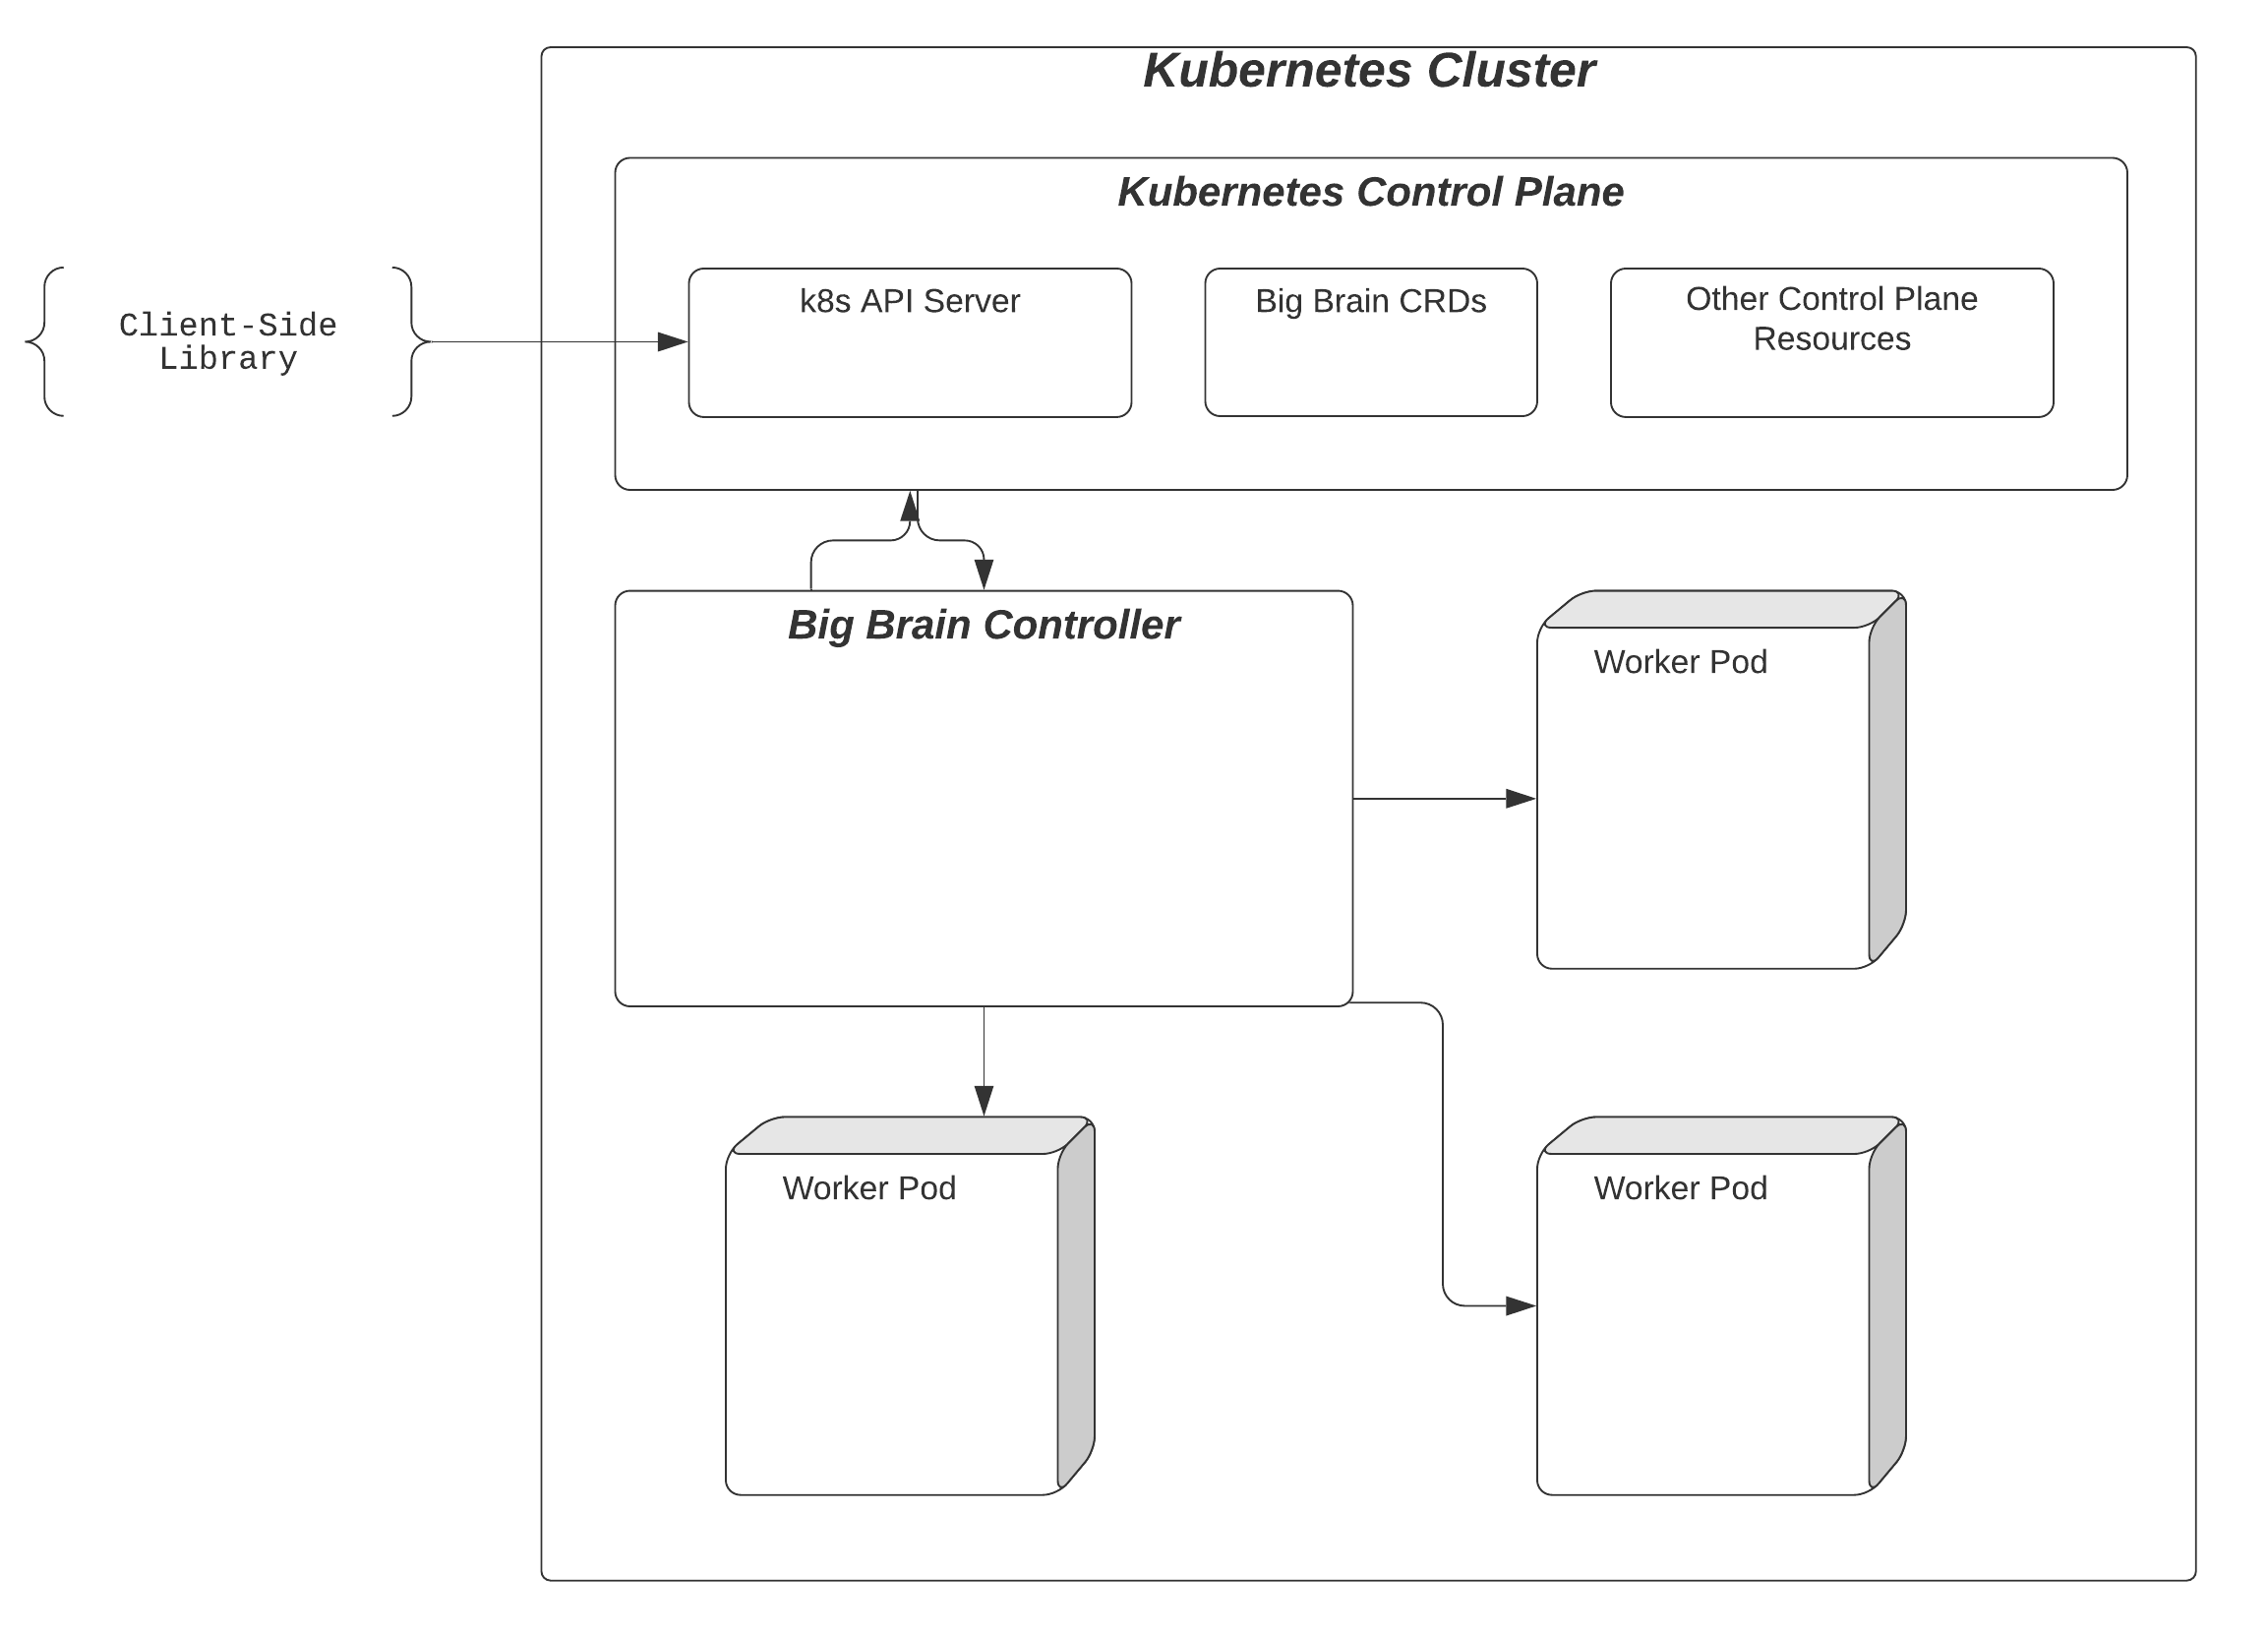
\includegraphics[height=5cm]{figures/architecure.png}}
\caption{Kubernetes system diagram}
\end{figure}

\subsection{Resource Management}

Two resources that matter for us are GPU compute and GPU memory. The safety
property we aim for is that GPU should never have an OOM error. So the scheduler
must be aware of available GPU memory at all times. A global resource manager
maintains the record of memory changes at all GPUs as jobs enter and leave. On
the other hand, it is difficult to keep track of the compute resource, since it
is handled by the GPUs internal scheduler and context handler. Allotting more
jobs than available compute does not lead to errors, but may cause severe
slowdown. Thus we had to control how many jobs are allotted to a GPU, even when
memory availability may allow it. This was simply done by having a tunable
parameter `packing factor' that scaled up the memory requirement of the job.
Thus greater the parameter, less jobs will be packed together. 

\subsection{Baechi}

Once a job is received, it is passed through a profiler. The profiler runs some
iterations of the training loop and constructs a graph. Nodes in the graph are
layers of the model. Nodes are tagged with the net memory requirement of that
layer and forward computation time. Edges show data dependency among the layers
and are tagged with the computation time (proportional to the size of data being
transferred). The graph and resource manager are then input into an LP solver to
get a good placement of layers across the GPUs [Details in Baechi paper]. The
model is then distributed across GPUs as per the placement and resource manager
is updated.

\begin{figure}[htbp]
\centerline{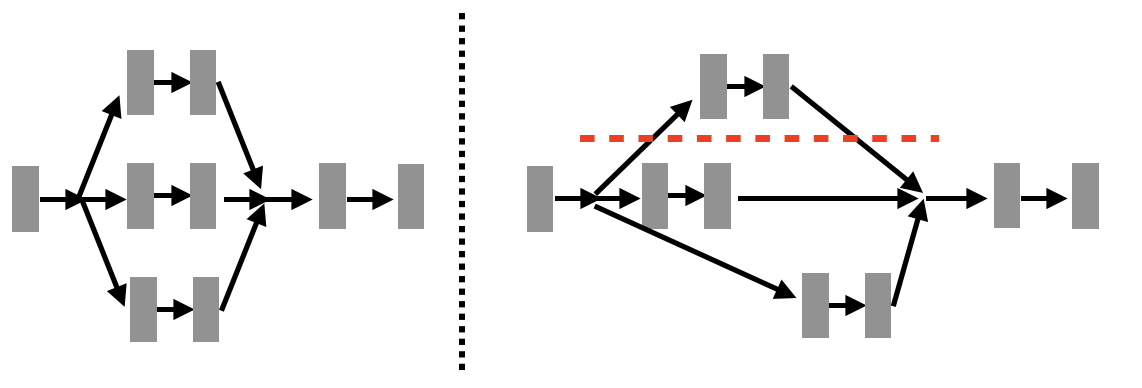
\includegraphics[height=3cm]{figures/layers.png}}
\caption{Job Model \& the model split}
\label{fig4}
\end{figure}

%\section{Implementation}
%\label{sec:implementation}
%\subsection{Kubebuilder}
%\subsection{Scheduler}
%The scheduler is written in python. PyTorch is used for deep learning jobs

\section{Experiments}
\label{sec:results}

\subsection{Setup}

The Scheduler is written in python, with PyTorch for defining the ML jobs.

Sharing a GPU among multiple processes is not without cost. Ideally, if the
compute units (cuda cores) of GPU are not saturated then two processes launched
together must execute in parallel. However, this is not true in practice because
each process has its own context and the GPU can operate within only one context
at a time. Therefore, execution of two processes can be serial in nature (though
entire detail is not in public domain). Thus, sharing GPU increases the
execution time for all the processes involved. This is has been studied
previously as in \cite{gandiva}. On the other hand, if the GPU were not shared,
the jobs would be waiting in the queue. There is a tradeoff between waiting time
and processing time. 

We assume incoming jobs are all training jobs for the model shown in Figure 4.
Jobs arrive as a Poisson process. The model has only linear layers. When a job arrives, based on the resource available,  Baechi creates a model split for the incoming model. 

We had two experimental setups. One of them had 4 GeForce RTX 2080 with 8GB memory each. Other had two RTX 3090 Founders Edition GPUs with 40GB memory each.

%In summary, we built a toy emulator that can handle one type of job with two
%possible placements. The job queue and scheduler are implemented in Python.
%Kubernetes is used to manage the cluster and Docker is used to package the job
%(one for each kind of \texttt{train.py}). We note that in Kubernetes if no GPU
%resources are mentioned in the configuration YAML of the job, then job has
%access to all the GPUs on the machine the job is scheduled. Thus we specify no
%GPU resources and this allows us to pack jobs in GPU without involving
%Kubernetes to allot GPUs to jobs (which would be in integers). But this also
%means that the scheduler takes care not to cause Out-Of-Memory error on the GPU
%by allotting more jobs than it can handle. Our setup consists of only one node
%with two RTX 3090 Founders Edition GPUs.

\subsection{Key Questions and Results}

The key question we had to answer for this project was: \emph{Is it ever beneficial to share GPU among multiple jobs?}

\emph{We found that under no scenario, sharing jobs on a GPU is beneficial, except when the underlying hardware itself supports granular compute resource allocation (eg: Multi-instance GPUs, Multi-process services).} In particular we considered these scenarios:

\subsubsection{Simple Packing}

In simple packing, we pack entire training jobs, without splitting the model across GPUs. The result is for a 100 sec run with 3 available GPUs. Packing number indicates how many jobs can are allowed to be run on one GPU. So with packing number of 2 and with three GPUs, atmax 6 jobs can run simultaneously. For each case we measure, GPU utilization as shown by nvidia-smi, `Waiting Time' - the time between arrival of a job and when it is placed on a GPU, `Process Time' - the time from when job is placed on GPU to its completion. Jobs completed is the total number of jobs processed by the 3 GPUs in 100sec. The process time degrades almost proportionally to packing number, such that it cancels any advantage from simultaneous execution of jobs. Clearly, there is no advantage to packing more. Further, as shown in Figure 5, on packing more, the variation in process time increases thus making the system more unpredictable.

\subsubsection{Parallel Models}
One scenario in which simultaneous execution might be expected to help is in case of highly parallel deep learning models. Consider the model shown in Figure 4. Splitting the model across two devices along the red line executes faster than on a single device. Thus if there are two such jobs, then we might expect that dividing each job across both the GPUs might be faster than allotting one job per GPU. However this is not true either. Process time degradation eliminates any advantage. Since all jobs are launched from the same process (as different threads), there should not be any context switching costs. However, all tasks are placed in to a default stream by the GPU and is thus serialized on the GPU.

\subsubsection{Use of streams}
Streams are the basic primitive for parallel task execution on a GPU. So we might expect that launching each job on a new stream would be advantageous. However, this is not observed, because streams only interleave execution of two jobs. It does ensure their concurrent execution

Thus unless there is hardware support for simultaneous execution of tasks, sharing GPU's across job is not useful.



%`Concurrency Factor' is number of entire jobs that are allowed to be packed in
%to a GPU. Thus a factor of 2 means upto 2 full jobs can run on a GPU. Thus with
%2 GPUs, at most four jobs and one job split across the GPUs can run at a time.
%For a given factor, we run for the experiment for 30 sec with a job arrival rate
%enough to keep the GPUs always occupied. We measure the mean and max process
%time among all the jobs that ran during the 30 sec interval. The result is
%plotted in Figure 5.
\vspace{0.5cm}
\begin{tabular}{ |p{3cm}||p{1cm}|p{1cm}|p{1cm}|  }
 \hline
 \multicolumn{4}{|c|}{Experiment Duration = 100 sec} \\
 \hline
 Packing Number & 1 & 2& 3\\
 \hline
 Utilization   & 17-20\%    & 18-22\%  &   19-22\%  \\
 Waiting Time(s)   & 12.44    &13.27&   11.58\\
 Process Time(s)&  4.58  & 8.97   & 13.82\\
 Net Time(s) &17.02 & 22.24&  25.41\\
 Jobs Completed    &59 & 61&  59\\
 \hline
\end{tabular}

\begin{figure}[htbp]
\centerline{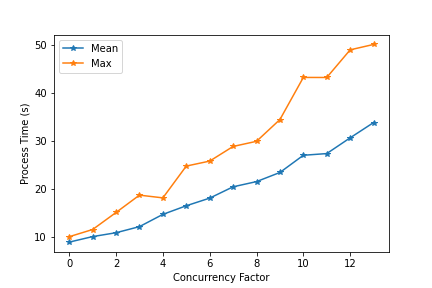
\includegraphics[height=5cm]{figures/graph.png}}
\caption{Results}
\label{fig5}
\end{figure}

In light of these observations, we are curious about benfits of project like \cite{ali} (from Alicloud). They explicitly say they don't solve for isolation among jobs sharing a GPU. In which case, we have observed no speed or utilization advantage.

\subsubsection{Multi-process Service (MPS)}
One such hardware support is MPS. We used the two-GPU node to run jobs split across the two GPUs.Having the MPS on gave about 12\% in the training speed, which is much less the expected ideal 100\% speedup. We have not explored the reasons for the same in depth yet. \\

%One job uses about 25\% of a GPUs compute resource. One would thus expect upto 4
%process to run on a GPU without affecting each others process-times. However
%this is clearly not true as shown in Figure 5. Process time increases linearly
%with the concurrency factor. Further, the variance of the process times also
%increases as in clear from the max plot (orange). Thus packing of the GPU has
%diminishing returns and we should find a sweet spot that balances the process
%time degradation with job queue waiting time.

%\section{Future Work}
%\label{sec:future_work}     
%
%Based on the observations above, the immediate next step is to incorporate
%better process sharing in a GPU. We note that Nvidia's Multi-Process Service
%(MPS) provides for this. We will be integrating Baechi into the setup discussed
%above. This would allow us to run the same experiment with a realistic and
%diverse workload. The observations would guide us in adding the intelligence
%layer in the scheduler that can free the developer from having to deal with the
%hardware. For example, given a model, is it better to split it across available
%GPUs or wait until an entire GPU is free.
